\documentclass[11pt]{article}
\usepackage{fullpage}
\usepackage{graphicx}
\usepackage{tikz}
\usepackage{hyperref}

\title{CS63 Fall 2022\\Lab 5: Explaining XOR Network}
\author{\ldots}%TODO: replace \ldots with your names

\begin{document}

\maketitle

With random seed \ldots %TODO: replace \ldots with your seed
the XOR network achieved 100\% accuracy on the XOR data set after
\ldots %TODO: replace ldots with epochs
training epochs.  The resulting neural network is shown in the
following diagram.

%TODO: fill in the weights with ONE DECIMAL DIGIT of precision
\begin{center}
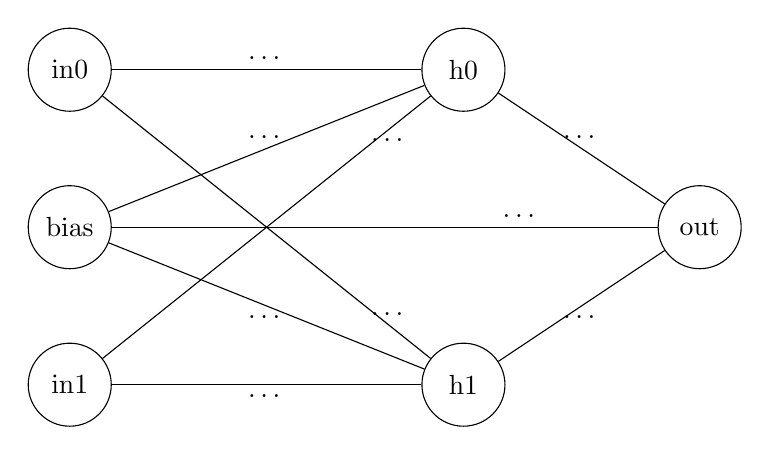
\begin{tikzpicture}
\tikzstyle{neuron}=[draw, circle, minimum size=30pt]

\draw (0,2) node[neuron] (bias) {bias};
\draw (0,4) node[neuron] (in0) {in0};
\draw (0,0) node[neuron] (in1) {in1};
\draw (5,4) node[neuron] (h0) {h0};
\draw (5,0) node[neuron] (h1) {h1};
\draw (8,2) node[neuron] (out) {out};

\draw (in0) edge node[above] {\ldots} (h0);
\draw (in0) edge node[very near end, above] {\ldots} (h1);
\draw (in1) edge node[very near end, below] {\ldots} (h0);
\draw (in1) edge node[below] {\ldots} (h1);
\draw (h0) edge node[above] {\ldots} (out);
\draw (h1) edge node[below] {\ldots} (out);
\draw (bias) edge node[above] {\ldots} (h0);
\draw (bias) edge node[below] {\ldots} (h1);
\draw (bias) edge node[near end, above] {\ldots} (out);
\end{tikzpicture}
\end{center}

Based on these weights, this network solves XOR as follows.

% TODO: Explain how the network solved the XOR problem based on these
% parameters.

 

\end{document}
